\begin{figure}[t]
\cite{Cave:2011:HNA:2093157.2093165}
\centering
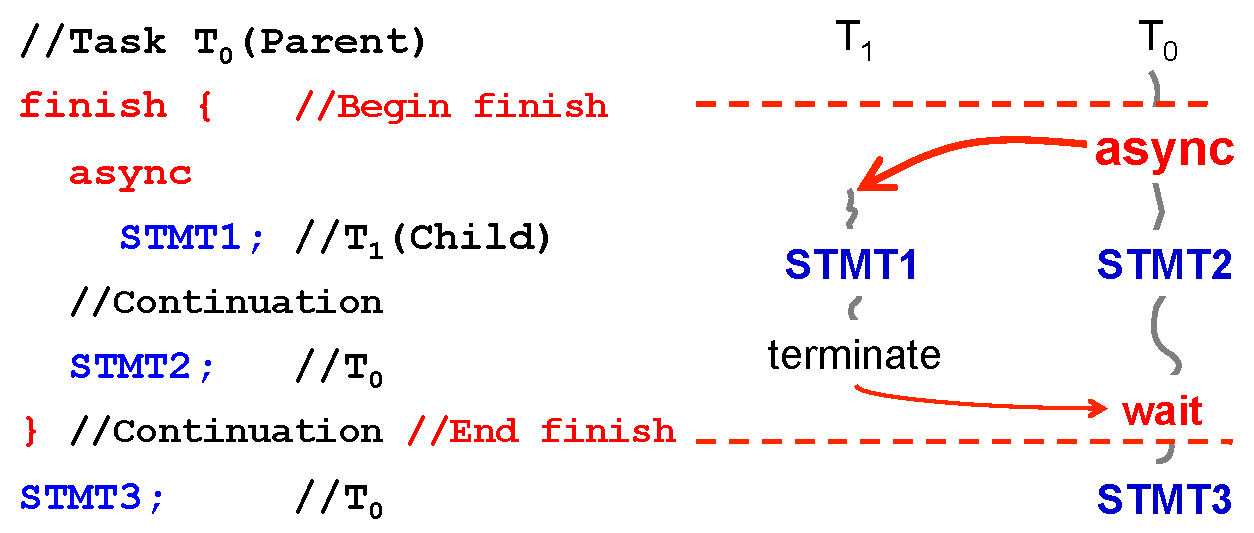
\includegraphics[width=3.25in]{../figs/async-finish}
\caption{An example with {\tt async} and {\tt finish}.}
\label{fig:async-finish}
\end{figure}

\begin{figure}[t]
\centering
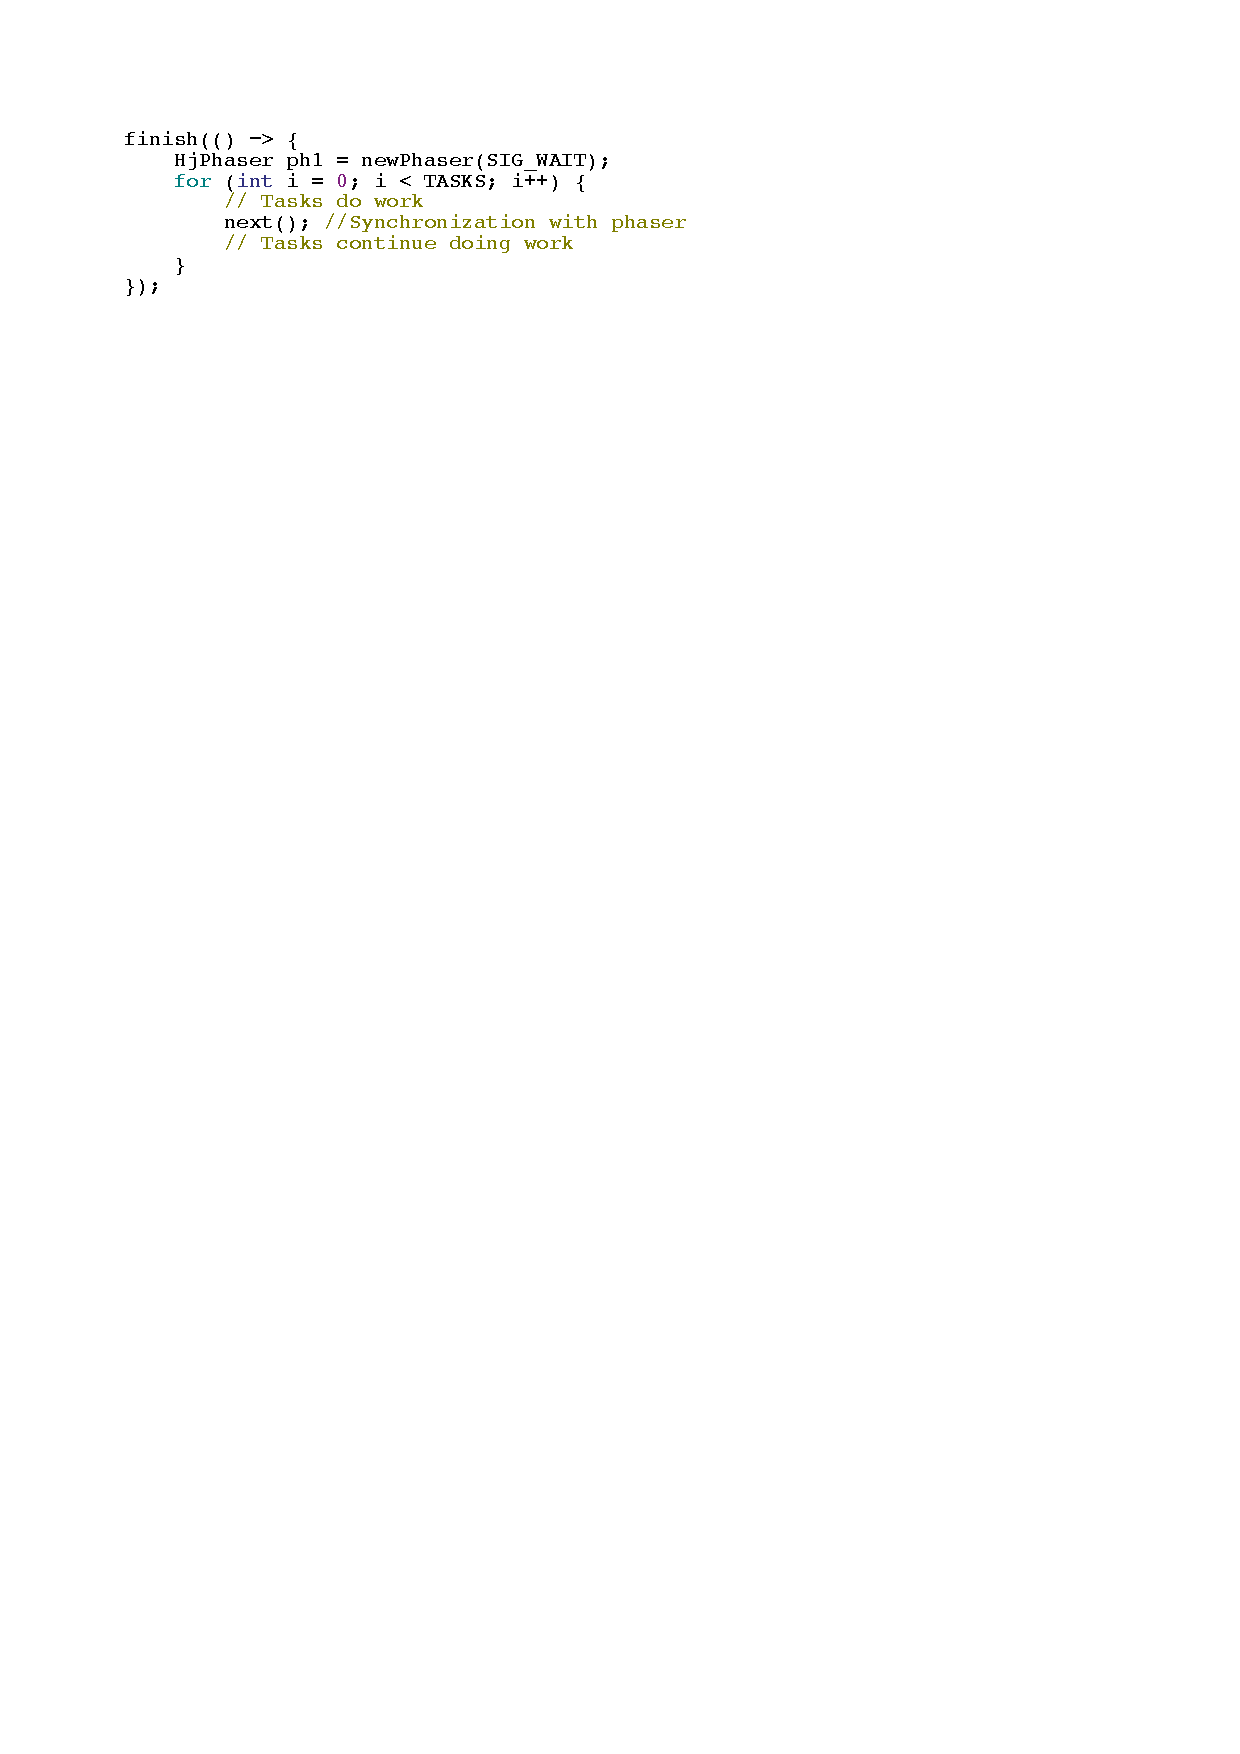
\includegraphics[width=3.25in]{../figs/phaser-example}
\caption{Use of phasers to mimic barrier behavior}
\label{fig:phaser-example}
\end{figure}

\begin{figure}[t]
\centering
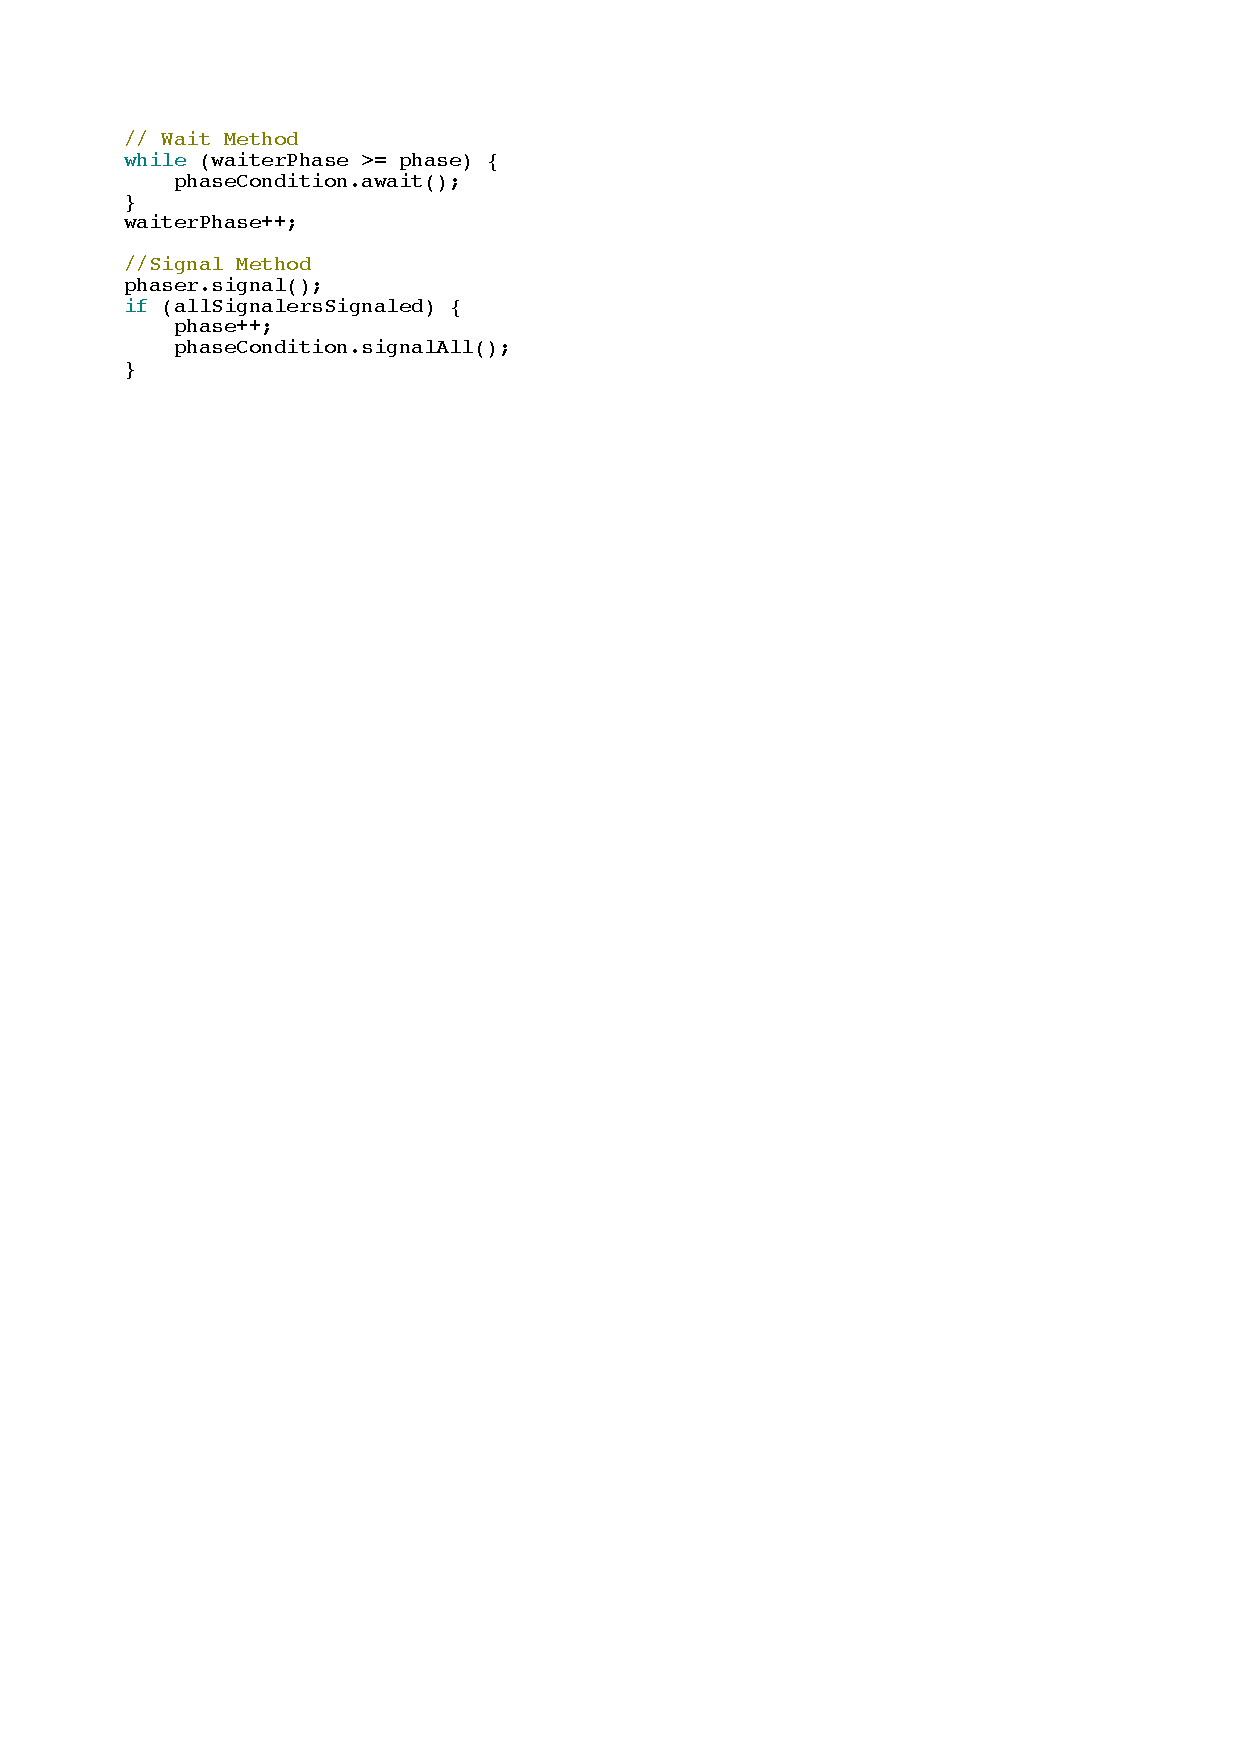
\includegraphics[width=3.25in]{../figs/sig-wait-impl}
\caption{Implementation of signalers and waiters using conditional locks}
\label{fig:sig-wait-impl}
\end{figure}

\section{habanero overview}

The Habanero Java library supports asynchronous tasking, collective
synchronization, mutual exclusion, message passing, and point-to-point
synchronization with async, finish, isolated, actors, and phasers
respectively \cite{hj-lib}. Each of these primitives is accessed via library calls in
HJ-lib. A brief description of each primitive is provided below, followed by a more
thorough description for phasers. A more detailed description of all HJ
primitives can be found in \cite{Cave:2011:HNA:2093157.2093165,
shirako:2008:pud:1375527.1375568}. 
% NV: using a different font to distinguish code from text would be good.
% Also, it's not clear what "async: async(hjrunnable);" is supposed to mean.
\begin{compactitem}
\item async: async(hjrunnable); generates an asynchronous task that executes the
statements in the run method of the hjrunnable object,
which can be specified succinctly in Java 8 as a lambda expression.
See \figref{fig:async-finish} for the execution semantics.
\item finish: finish(hjsuspendable); collects all spawned tasks generated in the
body of the run method (or lambda) for hjsuspendable. As indicated in figure
\figref{fig:async-finish}, a finish construct waits for all asyncs in its scope
to complete before transferring control to the continuation following the call
to finish().
\item isolated: isolated(hjrunnable); provides a guarantee that all interfering
isolated regions will be executed in mutual exclusion. Interfering regions are
defined as regions that access the same object with at least one of the regions
containing a write-access.
\item phasers: newPhaser(HjPhaserMode); creates a new phaser and registers the
calling task with registration mode given by HjPhaserMode. Four possible modes
are available: {\tt signal}, {\tt signal-wait}, {\tt wait}, and {\tt
signal-wait-next} with each modifying the synchronization behavior of the
registered task in relation to the newly created phaser. Variants of the async
API enable a child task to be registered on a subset of phasers that the parent
task is registered on. 
\end{compactitem} 

Phasers extend barriers as a form of synchronization. They order execution of
portions of the program into phases. Like barriers, they can restrict tasks from
executing the next phase until the current phase is complete. However, unlike
barriers, phasers allow tasks to specify point-to-point relationships on
multiple phases.

All tasks that have designated themselves as signalers must signal the phaser
in order for the phase to advanced.  

Waiters are required to stop at the phaser until the phase has been advanced.
The exception to this rule are waiters that are registered on bounded phasers,
in which the bound specifies a permissible "slack" in number of phases between
waiters and signalers. 

Signaler-Waiters function as both a signaler and a waiter. A phaser that has
only signaler-waiters registered to it will function much like a traditional
barrier (except that phasers allow tasks to dynamically join or leave the
barrier.) \figref{fig:phaser-example} illustrates the use of phasers as
barriers.

For both signalers and waiters, synchronization is performed by a "next" call to
the library. The next operation causes signalers to signal, waiters to wait, and
signalers-waiters to do both.

VR-lib implements phasers using lock condition variables, as seen in
\figref{fig:sig-wait-impl}. Tasks registered as waiters wait on the lock until
the condition is satisfied (all registered signalers have signaled for the
% NV: Two things here. 1) This is the first time I get the impression that VR-lib
% is an alternate implementation of HJ-lib. I thought VR-lib was just the JPF
% stuff for supporting your implementation of HJ-lib.
respective phase). In VR-lib each Habanero task is represented
as a thread. Thus we rely upon JPF's native scheduling of threads to explore all
schedules introduced by the phaser.
